\chapter{Introducción}
\label{cap:introduccion}

Una misma escena se ve de manera diferente según la cámara que la observe. La cámara común forma la
imagen con la luz que reflejan las superficies; por eso recoge el color y la textura. La cámara térmica
mide, en cambio, la radiación infrarroja que emite cada cuerpo según su temperatura. Gracias a eso, una
persona o un vehículo con el motor caliente resaltan sobre el fondo aun de noche o entre el humo. A
cambio, la imagen térmica pierde buena parte de esa textura. Ninguna de las dos cámaras basta por sí
sola en todas las condiciones. La fusión de imágenes infrarrojas y visibles combina ambas fuentes en una
sola imagen que conserve lo útil de cada una \parencite{ma2019}.

La Figura~\ref{fig:modalidades} muestra una escena nocturna en sus dos imágenes, la visible y la
infrarroja, junto con la que resulta de fusionarlas con el algoritmo que propone este trabajo. En la
imagen visible se distinguen los arbustos, el empedrado y la entrada del edificio, pero la persona que
camina junto a la entrada se confunde con los arbustos que tiene detrás. En la infrarroja, la persona
resalta en blanco, mientras el follaje queda oscuro y casi sin textura. La imagen fusionada conserva a la
vez la figura de la persona y la textura del fondo.

\begin{figure}[htbp]
\centering
\caption{Escena nocturna en la imagen visible, en la infrarroja y fusionada con el algoritmo propuesto}
\label{fig:modalidades}
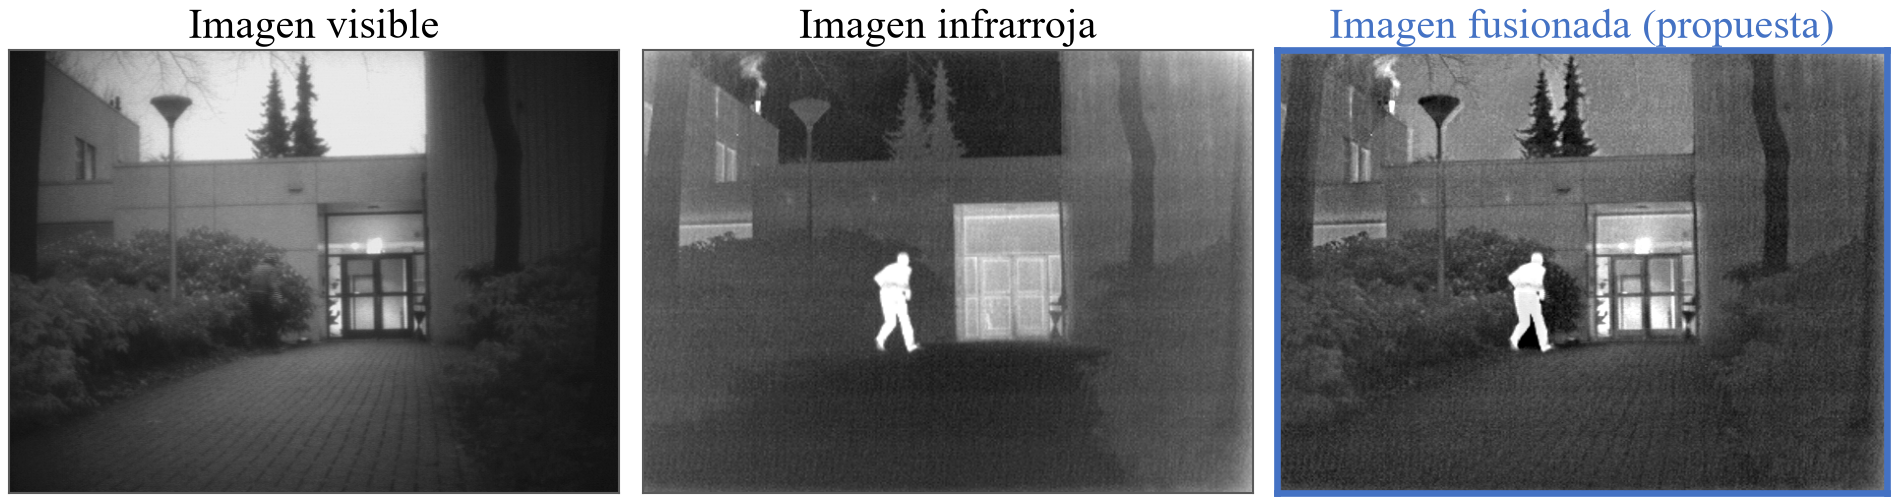
\includegraphics[width=\textwidth]{figuras/fig_modalidades}
\nota{Elaboración propia a partir de imágenes del conjunto de \textcite{toet2014, toet2017}. La escena
corresponde al par Kaptein 1123, uno de los veinte con que se evalúa la calidad
(Sección~\ref{sec:corpus}). La imagen fusionada, recuadrada a la derecha, se obtuvo con la configuración
adoptada, radio $r = 25$ y peso $m = 0.30$ (Sección~\ref{sec:ajuste}). La
Figura~\ref{fig:montaje_kaptein} muestra la misma escena fusionada con los demás métodos del estudio.}
\end{figure}

Los métodos de fusión se agrupan en varias familias \parencite{li2017, singh2023}. Los multiescala, como
las pirámides y las transformadas \textit{wavelet}, descomponen cada fuente en capas según el tamaño
del detalle, combinan las capas y reconstruyen la imagen. Otros recurren a representaciones dispersas,
que describen cada región con pocos elementos de un diccionario. Los más recientes emplean redes
neuronales que aprenden la regla de fusión a partir de ejemplos. La morfología matemática ofrece un
camino distinto.
Sus operadores recorren la imagen con una forma pequeña, el elemento estructurante, y la transforman
según cómo esa forma encaja en cada región. Con ellos, la transformada Top-Hat separa del fondo los
detalles claros u oscuros más pequeños que el elemento \parencite{soille2003, gonzalez2018}. Esa
separación ya se aprovechó para fusionar imágenes infrarrojas y visibles \parencite{bai2013, roman2020,
bajacfigueredo2024}.

Este trabajo propone un algoritmo de fusión de imágenes infrarrojas y visibles basado en morfología
matemática. Su núcleo es un operador Top-Hat de una sola escala. En lugar de un único elemento
estructurante, emplea un banco de cinco: un disco y cuatro segmentos lineales orientados a $0^\circ$,
$45^\circ$, $90^\circ$ y $135^\circ$. El detalle de cada fuente es la suma de lo que extrae el disco
y el promedio de lo que extraen los cuatro segmentos. La regla de fusión parte del promedio de las
dos fuentes, le suma el detalle claro y le resta el oscuro. Un peso $m$ regula cuánto detalle se agrega.
El algoritmo queda así definido por dos parámetros: el radio $r$ de los elementos y el peso $m$. Ambos se
ajustan mediante optimización por enjambre de partículas. En esa búsqueda, un grupo de soluciones
candidatas recorre el espacio de los parámetros, guiado por las mejores posiciones halladas. En las
veinticinco corridas del enjambre, el peso terminó en 0.30, que es el límite inferior del rango de búsqueda. El
radio quedó casi siempre en 1 o en 25 píxeles. De esos dos valores se adoptó $r = 25$, porque prioriza
el realce: da más contraste y nitidez que $r = 1$, a cambio de una imagen menos fiel a las fuentes.

El problema que aborda la tesis tiene dos partes. La primera se refiere a la calidad: si las imágenes del
algoritmo propuesto están a la altura de las que producen los métodos clásicos de fusión. Como
referencia se toman el Top-Hat clásico, que aplica la misma regla con un único disco, y cinco métodos
multiescala: dos pirámides y tres transformadas \textit{wavelet}. La segunda parte es la aplicación: si
esas imágenes ayudan a un detector automático a encontrar objetos. La variable que se manipula es el
método de fusión; las que se miden son la calidad de la imagen y el acierto del detector.

Medir la calidad tiene una dificultad propia, porque no existe una imagen fusionada ideal con la cual
comparar. Por eso se recurre a métricas sin referencia, que prescinden de ella pero no siempre coinciden
entre sí. El trabajo de \textcite{bajacfigueredo2024}, en el que participaron los
autores de esta tesis, ilustra ese desacuerdo. En la escena Camp, con elementos estructurantes de tamaños
7 y 9, la fusión con Top-Hat de ese trabajo quedó primera en desviación estándar, entropía y frecuencia
espacial, que miden el contraste, la información y la nitidez. Al mismo tiempo quedó última en
información mutua, que mide el parecido con las fuentes.

La propuesta reúne piezas que provienen de trabajos distintos. El banco de cinco elementos
estructurantes se diseñó para realzar el contraste local y la nitidez en mamografías \parencite{floressf}.
La forma de combinar las respuestas del disco y de los segmentos se tomó de un método de realce de
imágenes de fondo de ojo \parencite{bala2024}. La regla de fusión con un peso y el ajuste del radio y del
peso por enjambre de partículas provienen de \textcite{ortegarodriguez2025}, que trabajaron con un único
disco. El Top-Hat clásico sigue la fusión con Top-Hat del trabajo ya citado
\parencite{bajacfigueredo2024} y se aplica aquí con un disco de radio 5 y peso 1. En la literatura
revisada no se encontró el banco aplicado a la fusión de imágenes infrarrojas y visibles. El aporte de
la tesis es llevarlo a esa fusión, junto con el ajuste de sus parámetros. Sobre esa base se
caracteriza la calidad de las imágenes resultantes y se evalúa la aplicación del algoritmo a la
detección. A diferencia
de una red neuronal, un operador morfológico puede explicarse paso a paso. Esa transparencia permite relacionar lo que premia cada métrica con lo
que hace la regla de fusión.

Las métricas de imagen dicen poco sobre lo que la fusión aporta a un uso concreto. Por eso, trabajos
recientes la evalúan también por su efecto en una tarea posterior, como la detección o la segmentación
de objetos \parencite{liu2022, tang2022}. Un detector que recibe la imagen fusionada debería encontrar
en ella lo que cada cámara muestra por separado. Un peatón en la sombra y un farol encendido ilustran el
caso. Al primero lo ve casi solo la cámara térmica; al segundo, casi solo la común. En la aplicación, la
propuesta se compara con el Top-Hat clásico, que pertenece a la misma familia y usa la misma regla.
Así, la comparación mide el efecto de cambiar el operador en su conjunto, con sus elementos
estructurantes, su radio y su peso.

Se plantean, en consecuencia, dos preguntas de investigación, una sobre la calidad de la fusión y otra
sobre su aplicación. ¿Qué calidad tienen las imágenes del algoritmo propuesto, frente al Top-Hat clásico
y a cinco métodos multiescala? ¿Encuentra un detector entrenado con esas imágenes más objetos vistos por
una sola cámara que uno entrenado con las del Top-Hat clásico?

La hipótesis del trabajo es la siguiente.

El algoritmo de fusión propuesto, con sus parámetros ajustados mediante optimización por enjambre de
partículas, produce imágenes de mejor calidad que el Top-Hat clásico y de calidad comparable a la de
cinco métodos multiescala, medida con seis métricas sin referencia. En su aplicación a la detección de
objetos, un detector entrenado con sus imágenes encuentra más objetos vistos por una sola cámara que el
entrenado con las imágenes del Top-Hat clásico.

Las dos oraciones de la hipótesis reúnen tres afirmaciones: dos sobre la calidad (frente al Top-Hat
clásico y frente a los métodos multiescala) y una sobre la aplicación a la detección. Cada una se examina
con las pruebas de la evaluación que le corresponde, sin agregar otras (Sección~\ref{sec:examen-hipotesis}).

El trabajo se sitúa en el año 2026 y se desarrolló en el marco de la Maestría en Ciencia de Datos de la
Universidad Comunera. Sus beneficiarios son, en primer lugar, los investigadores en procesamiento de
imágenes, que disponen de un operador morfológico descrito paso a paso y comparado con métodos
establecidos. También lo son quienes desarrollan sistemas de vigilancia o de detección con cámaras
visibles y térmicas y deben decidir cómo fusionar sus imágenes.

\section{Objetivos del trabajo}
\label{sec:objetivos}

\subsection{Objetivo general}

Proponer un algoritmo de fusión de imágenes infrarrojas y visibles basado en morfología matemática, con
sus parámetros ajustados mediante optimización por enjambre de partículas, y evaluar la calidad de sus
imágenes y su aplicación a la detección de objetos.

\subsection{Objetivos específicos}

Para alcanzar el objetivo general se plantean cuatro objetivos específicos. Las conclusiones del
Capítulo~\ref{cap:conclusiones} los retoman en el mismo orden.

\begin{itemize}
\item Implementar el algoritmo propuesto y ajustar su radio y su peso mediante optimización por enjambre
de partículas.
\item Evaluar la calidad de sus imágenes con seis métricas sin referencia y pruebas estadísticas no
paramétricas, frente al Top-Hat clásico y a cinco métodos multiescala.
\item Evaluar su aplicación a la detección de objetos vistos por una sola cámara, frente al Top-Hat
clásico, con detectores entrenados sobre cada tipo de imagen.
\item Examinar la hipótesis con los resultados de las dos evaluaciones.
\end{itemize}

\section{Alcance y delimitaciones}
\label{sec:limitaciones}

Los resultados del estudio deben leerse dentro de los límites siguientes:

\begin{itemize}
\item \textbf{Validez interna:} Las métricas sin referencia premian propiedades distintas de la imagen,
de modo que el orden entre los métodos depende del conjunto de métricas elegido. Los métodos
comparativos se aplican con sus parámetros por defecto, sin ajuste. En cambio, la aptitud del enjambre
se calculó sobre tres de los veinte pares con que se evalúa la calidad, y el radio se eligió entre los
dos que dio el enjambre comparándolos sobre los veinte.
\item \textbf{Detección:} Los detectores entrenados con cada cámara, y no una revisión humana, definen
cuáles son los objetos vistos por una sola cámara. Los objetos de la prueba provienen de pocos tramos de video, y casi dos
de cada tres luces salen de un mismo grupo de tramos. Se emplea un solo modelo de detector, el más
pequeño de su familia, entrenado durante cuarenta épocas (pasadas completas por los datos de
entrenamiento).
\item \textbf{Validez externa:} La calidad se mide en veinte pares de un único conjunto, el
\textit{TNO Image Fusion Dataset} \parencite{toet2014, toet2017}. TNO es la sigla de la organización neerlandesa
de investigación científica aplicada (del neerlandés \textit{Nederlandse Organisatie voor Toegepast
Natuurwetenschappelijk Onderzoek}), que reunió las imágenes. En buena parte de esos pares, la imagen
visible proviene de cámaras con intensificador de imagen, que amplifican la escasa luz disponible. La
detección se evalúa en otro conjunto, M3FD (del inglés \textit{Multi-scenario Multi-modality
Dataset}), con pares de escenas diurnas y nocturnas en los que los objetos están marcados
\parencite{liu2022}. De sus seis clases de objetos, el análisis se centra en dos, las personas y las
luces. La imagen visible se usa en escala de grises. El radio se expresa en píxeles y no se adapta al
tamaño de la imagen.
\item \textbf{Alcance:} El estudio usa solo conjuntos públicos, cuyos pares ya vienen registrados por sus
autores; el corrimiento vertical de varios píxeles que muestran algunos pares del TNO no se corrigió
(Sección~\ref{sec:corpus}). No incluye captura propia de imágenes, alineación de pares ni medición del tiempo de cómputo.
Su foco es un operador de una sola escala. Por eso quedan fuera, para trabajos futuros
(Capítulo~\ref{cap:recomendaciones}), la fusión con redes neuronales y los métodos morfológicos
multiescala de \textcite{bai2013} y \textcite{roman2020}.
\end{itemize}

\section{Estructura del documento}
\label{sec:estructura}

Después de esta introducción, el documento se organiza de la manera siguiente:

\begin{itemize}
\item El Capítulo~\ref{cap:marco} expone el marco teórico y conceptual. Parte de los conceptos básicos
sobre la imagen digital y la fusión. Trata después los métodos de fusión de imágenes visibles e
infrarrojas, la morfología matemática, las métricas sin referencia y las pruebas estadísticas. Siguen
la optimización por enjambre de partículas y la detección de objetos, y el capítulo
cierra con el estado del arte y la brecha existente.
\item El Capítulo~\ref{cap:metodologia} describe los conjuntos de imágenes, el algoritmo propuesto y el
ajuste de sus parámetros, las dos evaluaciones y el examen de la hipótesis.
\item El Capítulo~\ref{cap:resultados} presenta los resultados en ese mismo orden: la caracterización de
los conjuntos, el ajuste, la calidad de imagen con su análisis estadístico, la detección y el examen de
la hipótesis.
\item El Capítulo~\ref{cap:discusion} discute la calidad y su costo, el ajuste, la detección y la
relación entre ambas, y precisa las limitaciones del estudio.
\item El Capítulo~\ref{cap:conclusiones} presenta las conclusiones, una por cada objetivo específico.
\item El Capítulo~\ref{cap:recomendaciones} reúne las recomendaciones para trabajos futuros.
\item Los Anexos reúnen la participación de los autores en congresos y la tabla completa de los
contrastes de Wilcoxon (Tabla~\ref{tab:wilcoxon_completa}).
\end{itemize}
